\documentclass{../templates/topic}

\begin{document}
\graphicspath{{assets/}{ch2b_State_Space_Representation/assets/}}

\chapter{State Space Representation}

\begin{section}{Definition}
	\definition{State} The collection of variables which completely defines the present and future of the system
	
	\definition{State Space Equation} Equations which relate the state variables and input variables to the output variables. These will take the form of a Vector-Matrix Differential Equation.
	
	The equations take the form
	\begin{align}
		\dot{\vec{x}}&= A\vec{x}+Bu\\
		\vec{y}&= C\vec{x} + Du
	\end{align}
	
	The matrices above have names:\\
	\definition{A} state matrix \\
	\definition{B} input matrix \\
	\definition{C} output matrix \\
	\definition{D} direct transmission matrix
	
	These can be represented as a block diagram:
	
	\begin{figure}[H]
		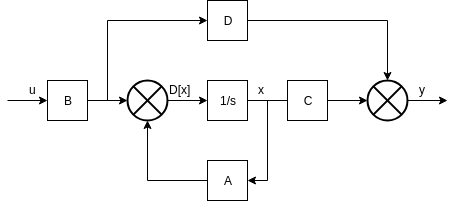
\includegraphics[width=\textwidth]{state_space_block_diagram.png}
		\caption{General Closed-Loop system block diagram}
	\end{figure}
	
	
\end{section}

\begin{section}{Characteristic Equation}
	The Characteristic Equation is the denominator of the TF and is given by
	\begin{equation}
		DET[s\vec1-A]
	\end{equation}
\end{section}

\begin{section}{State Transition Matrix}
	The STM is given as
	\begin{equation}
		\Phi(s)=INV(s\vec{1}-A)
	\end{equation}
\end{section}

\end{document}